\documentclass[tikz]{standalone}%

\usepackage[utf8]{inputenx}%  http://ctan.org/pkg/inputenx
% Euler for math | Palatino for rm | Helvetica for ss | Courier for tt
\renewcommand{\rmdefault}{ppl}% rm
\linespread{1.05}% Palatino needs more leading
\usepackage[scaled]{helvet}% ss //  http://ctan.org/pkg/helvet
\usepackage{courier}% tt // http://ctan.org/pkg/courier
\usepackage{eulervm}  %  http://ctan.org/pkg/eulervm
% a better implementation of the euler package (not in gwTeX)
\normalfont%
\usepackage[T1]{fontenc}%  http://ctan.org/pkg/fontenc
\usepackage{textcomp}%  http://ctan.org/pkg/textcomp

\usetikzlibrary{patterns}
\usetikzlibrary{intersections}
\usetikzlibrary{calc}
 
\begin{document}
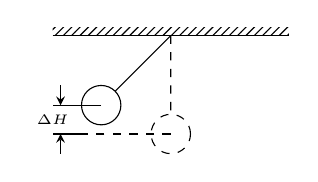
\begin{tikzpicture}
  \draw (-1.5cm, 0) -- (1.5cm, 0);

  \fill[pattern = north east lines] (-1.5cm, 0) rectangle (1.5cm, 0.1cm);

  \draw[dashed] (0, 0) coordinate (O) -- (0, -1cm) (0, -1.25cm)
  circle[radius = 0.25cm];
  \draw (O) -- (-135:1cm) (-135:1.25cm) circle[radius = 0.25cm];
  \draw[thick, dashed] (0, -1.25cm) -- (-1.1cm, -1.25cm) coordinate (P1);
  \draw[thick] (P1) -- (-1.5cm, -1.25cm) coordinate (P2);

  \begin{scope}
    \clip (-1.5cm, 0) rectangle (1.5cm, -1.5cm);
    \path[name path global = hline] (-135:1.25cm) -- +(-1cm, 0);
  \end{scope}

  \path[name path = vline] (-1.5cm, 0) -- (-1.5cm, -1.5cm);
  \path[name intersections = {of = hline and vline, by = P3}];

  \draw (-135:1.25cm) -- (P3);

  \node[font = \tiny] () at ($(P2)!.5!(P3)$) {$\Delta H$};

  \draw[stealth-] ($(P2) + (0.1cm, 0)$) -- +(0, -0.25cm);
  \draw[stealth-] ($(P3) + (0.1cm, 0)$) -- +(0, 0.25cm); 
\end{tikzpicture}
\end{document}
%%% Local Variables:
%%% mode: latex
%%% TeX-master: t
%%% End:
